\chapter{Thuật toán}
\section{Lọc cộng tác dựa trên mặt hàng (Item-based Collaborative Filtering)}
Phương pháp lọc cộng tác dựa trên mặt hàng so sánh người mua và đánh giá của họ đối với một tập mặt hàng nhất định. Thuật toán tính toán hàng xóm gần nhất của người mua. Mọi hàng xóm trước đã đánh giá mặt hàng được so sánh đến mặt hàng với độ tương đồng giữa các mặt hàng. Khi đa số các mặt hàng tương tự đã xác định. Sự dự đoán được tính toán bởi trung bình trọng số của các đánh giá của hàng xóm và độ tương tự của người đó và hàng xóm. Tính toán độ tương đồng của mặt hàng đã được làm với một vài phương thức bao gồm độ tương tự dựa trên cosine, độ tương tự đựa phép tương quan và độ tương đồng cosine điều chỉnh.
\subsection{Độ tương tự dựa trên Cosine (Cosine-based Similarity}
Cosine-based similarity là một phương pháp tính toán độ tương tự giữa các mặt hàng trong phương pháp lọc cộng tác dựa trên mặt hàng. Trong phương pháp này, một mặt hàng được biểu diễn giống một vector trong không gian người sử dụng. Góc giữa hai vector được tính và cosine của góc là độ tương tự của các mặt hàng. Cho ví dụ hai mặt hàng m và n được tính như sau:
\begin{center}
$similarities(m, n) = cosine(\bar{m},\bar{n}) = \frac{\bar{m}*\bar{n}}{||\bar{m}||_{2}*||\bar{n}||_{2}}$
\end{center}
Toán tử \" * \" biểu thị toán tử nhân giữa hai vector.

Tính toán độ tương tự dựa trên cosine có một khó khăn. Tỉ lệ đáng giá của người mua không được cân nhắc trong lúc tính toán. Tính toán được thực hiện qua thông tin từ một vài cột, và mỗi cột đại diện cho một người sử dụng khác. Vấn đề này có thể giải quyết với độ tương tự cosine điều chỉnh bằng cách trừ đi trung bình đánh giá của người mua đó ở mỗi cột đã đánh giá. Độ tương đồng của hai mặt hàng m và n, sử dụng độ tương tự cosine điều chỉnh là:
\begin{center}
$similarity(m, n) = \frac{\sum_{u\in U}(R_{u,m}-\bar{R}_{u})(R_{u,n}-\bar{R}_{u})}{\sqrt{(R_{u,m} - \bar{R}_u)^{2}} \sqrt{(R_{u,n} - \bar{R}_u)^{2}}}$
\end{center}
$R_{u,m}$ là đánh giá của người sử dụng u cho mặt hàng m.
$\bar{R}_{u}$ là đánh giá trung bình cho người mua u.

\subsection{Độ tương tự dựa trên tương quan {Correlation-based Similarity}}

Độ tương tự dựa trên tương quan giữa hai mặt hàng m và n được tính bằng tương quan Pearson. Độ tương quan Pearson cho mặt hàng m và n được đánh giá bởi một tập người sử dụng U được tính toán như sau:
\begin{center}
$similarity(m, n) = \frac{\sum_{u\in U}(R_{u,m}-\bar{R}_{m})(R_{u,n}-\bar{R}_{n})}{\sqrt{(R_{u,m} - \bar{R}_m)^{2}} \sqrt{(R_{u,n} - \bar{R}_n)^{2}}}$
\end{center}
$\bar{R}_{u}$ là trung bình đáng giá của người sử dụng u.
%%% Local Variables: 
%%% mode: latex
%%% TeX-master: "isae-report-template"
%%% End:
\subsection{Tính toán dự đoán} 
Tính toán dự đoán đạt được bởi một vài công nghệ. Một phương pháp đơn giản là tính toán tổng trọng số của một mặt hàng m cho người mua u bằng lấy tổng của tất cả đánh giá các mặt hàng của người mua u tương đồng với m. Mục đích của phương pháp này là để hiểu đánh giá của một người mua cho các mặt hàng mà tương đồng đến mặt hàng đó là một phương pháp thử để dự đoán các đánh giá. Tổng trọng số cho dự đoán một mặt hàng m của người mua u được tính như sau:
\begin{center}
$P_{u, m} = \frac{(\sum_{N}(s_{m,k}*R_{u,k})}{\sum_{N}(|s_{m,k}|)}$
\end{center}
$P_{u, m}$ là dự đoán đánh giá của mặt hàng m của người mua u 
$R_{u, k}$ là đánh giá của người mua u cho mặt hàng k
N là tập các mặt hàng tương tự với m
k là một phần tử của N
$s_{m, k}$ là độ tương tự của hai item m và k.

\section{FunkSVD}
FunkSVD là một thuật toán sử dụng phương pháp tìm thừa số ma trận, tên là phân tích giá trị riêng (SVD). Phân tích giá trị riêng được sử dụng để giảm một ma trận đến hai ma trận với số chiều ít hơn. Hai ma trận kết quả được sinh ra biểu diễn các mặt hàng và người mua. Dự đoán được tính bằng tích của một hoặc nhiều vector mặt hàng và một vector người sử dụng. Một ví dụ của phân tích giá trị riêng giảm một trận đến hai ma trận khác được biểu diễn trong hình dưới. Trong hình, ta thấy u1 to u4 biểu thị các người mua, i1 đến i3 biểu thị các mặt hàng và f1 đến f3 biểu thị tính năng. Các tính năng thường được gọi là nhân tố ẩn
\begin{center}
\begin{figure}[H]
	\centering
	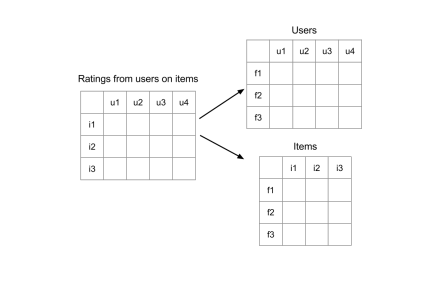
\includegraphics[width=1\textwidth]{svd.png}
	\caption{Singular value decomposition in a dataset}
	\label{fig:SVD}
\end{figure}
\end{center}
FunkSVD đào tạo ra một mô hình để đạt được độ chính xác nhất có thể cho các mặt hàng và người mua. Trong quá trình đào tạo, thuật toán có một tham số được gọi là số vòng lặp. Số vòng lặp thể hiện có bao nhiêu lần đào tạo cho một ô trong ma trận được cho là chạy. Số vòng lặp có thể là một số cố định hoặc tùy theo một số giới hạn khác để kết thúc vòng lặp.

Một ưu điểm của phân tích giá trị riêng là hai ma trận phân tích thường có ước lượng tốt hơn so với ma trận ban đầu. Mục đích của nhân tử ma trận là sinh ra dữ liệu bằng việc trích xuất sở thích người mua phổ biến, phân loại chúng để có được cái nhìn tổng quát của người mua.